\documentclass[a4paper,14pt]{article}

\usepackage[utf8]{inputenc}
\usepackage[english]{babel}
\usepackage{graphicx, array, blindtext}
\usepackage[colorinlistoftodos]{todonotes}

\usepackage{enumitem}
\usepackage{amsmath}
\usepackage{amsthm}

\usepackage{nameref}
\usepackage{amssymb}
\usepackage{xcolor}
\usepackage{floatrow}
\usepackage{cancel}
\usepackage{fancyhdr}
\usepackage{graphicx}
\usepackage{verbatim}
\usepackage[document]{ragged2e}

\rhead{CS765 Assignment 1}
\usepackage{subcaption}
\usepackage{listings}


\usepackage{hyperref}

\begin{document}
\centering{

\title{\fontsize{150}{60}{CS765 Assignment 1}}

\author{
Prathamesh Pilkhane\\
Shashwat Garg \\
Vedang Asgaonkar}
}

\date{Spring 2023}
\maketitle

\justifying

% \tableofcontents
% \newpage

\justifying

\section*{Introduction}

Hello and Welcome to our CS765 Project part 1. We have developed a simulator of a P2P Blockchain network using python.\\
This document will go over the design and structure of the code, answers to the questions in the assingment and some results obtained by visualising the data obtained from the network.

\section{Code Flow}

The code implements a simulation of a cryptocurrency network, where there are $n$ nodes and each node is represented by the Node class.\\
The simulation is initialized by the \verb|initialize_nodes| function, which generates random degrees and connections for the nodes, sets their initial properties (such as the number of coins they have), and initializes their blockchains with a Genesis Block.\\
The simulation is then run by inserting various events (transactions and block events) into a priority queue (implemented as PriorityQueue).\\
The events are processed in order of priority, with each event modifying the state of the network and potentially leading to the creation of new events.\\
The simulation ends when there are no more events left in the priority queue. The logs of the transactions and blocks are recorded in the 'txns\_log.txt' and 'block\_log.txt' files.

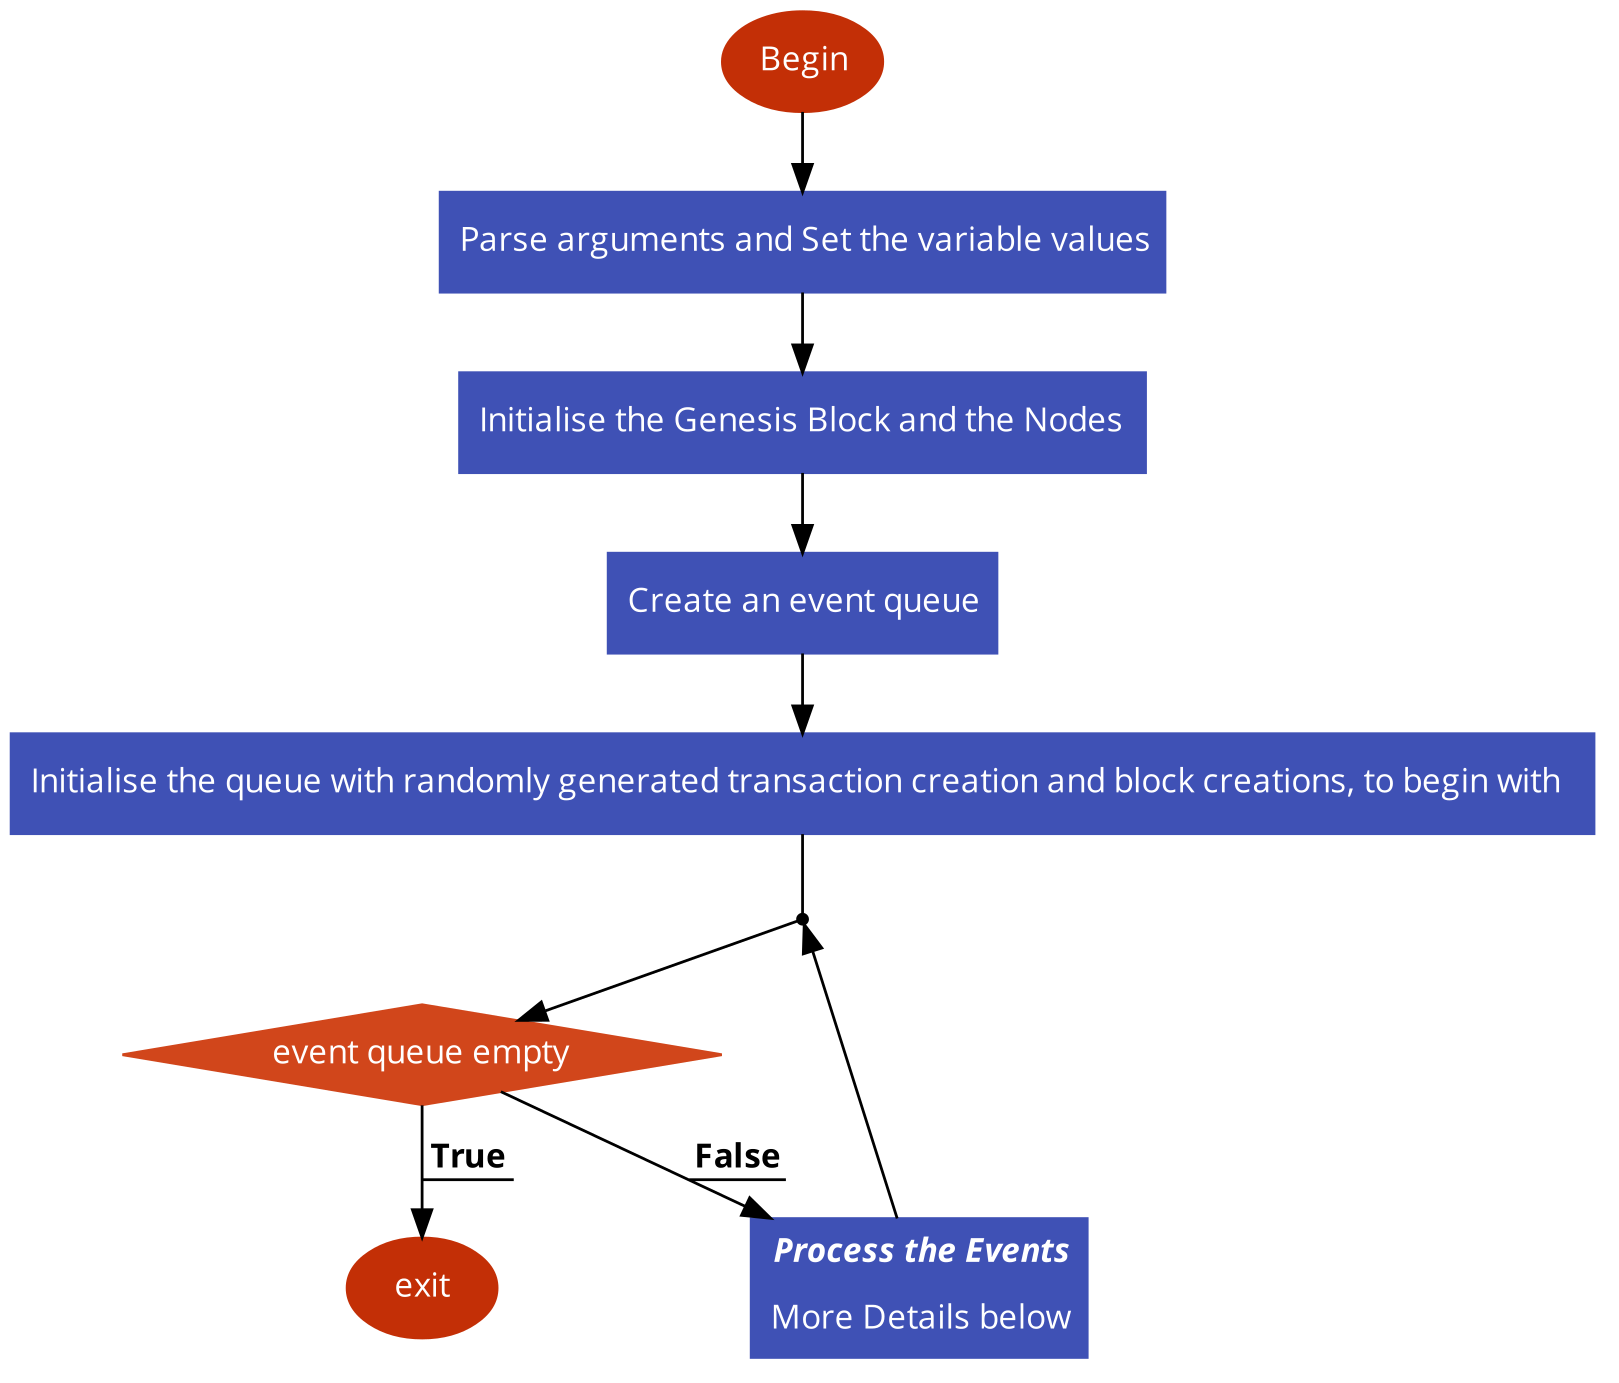
\includegraphics[width=10cm]{CodeFlow.png}

\section{Objects- Transactions, Blocks and Nodes}

The \verb|Transaction| class is used to store information related to transactions on the blockchain network. It has attributes such as ID, sender\_id, receiver\_id, size of transaction and the number of coins being sent

The \verb|Block| class is used to represent a block in the blockchain, and it has several attributes such as its ID, transactions, state of the network, depth in the blockchain, and the ID of its creator.

The \verb|Node| class represents a node in the network, and it has several attributes such as its ID, connections to other nodes, all the transactions it has seen, and its blockchain information. \\
The Node class has methods such as \verb|initialize_blockchain| to initialize its blockchain, \verb|_walk_blockchain| to return a generator of blocks from the head to the Genesis block, \verb|_verify| to verify a block's transactions, and \verb|insert_block| to insert a block into the node's blockchain after verification.

\section{Events}

The distributed system of nodes generate transactions and blocks, broadcast transactions and resolve conflicts between blocks. The main simulation logic is in the \verb|trigger| method of each event class.

The \verb|Event| class is the base class for all events in the simulation and is decorated with the \verb|functools.total_ordering| class decorator, which provides the necessary ordering method implementations for the class to be used with the priority queue (i.e., the heapq module).

The \verb|TransactionEvent| class creates a new transaction and schedules its broadcast to all peers using the \verb|BroadcastTransactionEvent|. It also schedules the next transaction to be done by the sender node.

The \verb|BroadcastTransactionEvent| class broadcasts the transaction to all of its neighbors, and if the transaction has not been seen by a neighbor, schedules a new \verb|BroadcastTransactionEvent| for that neighbor.

The \verb|BlockEvent| class generates a new block based on the block parameters provided, and triggers the process of validating the block and adding it to the local blockchain. If the block is valid, the node generates a \verb|BroadcastBlockEvent| to broadcast the new block to its neighbors.

Depending on the event, here are the actions taken.

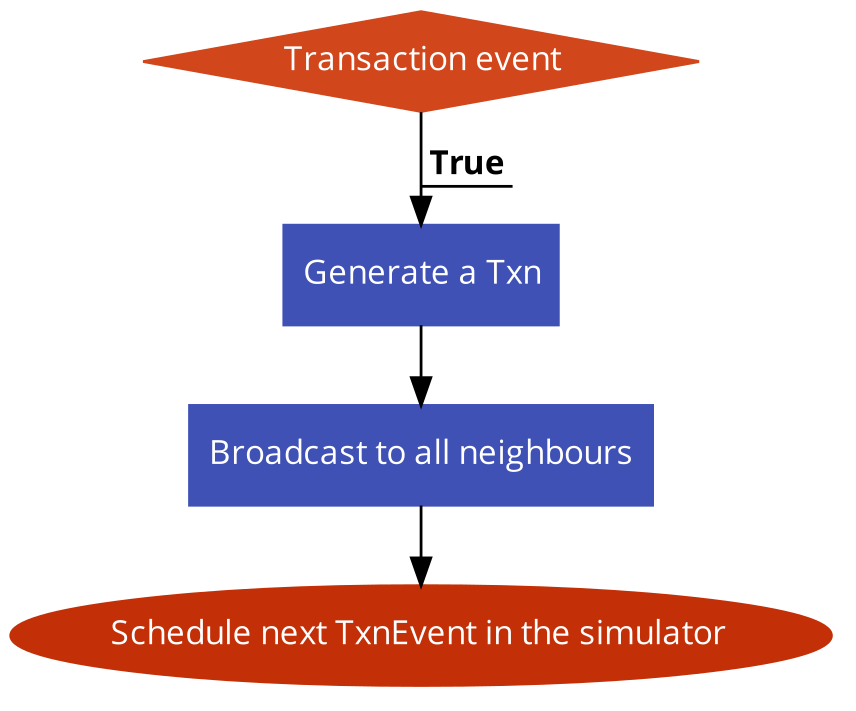
\includegraphics[width=6cm]{Txn.png}
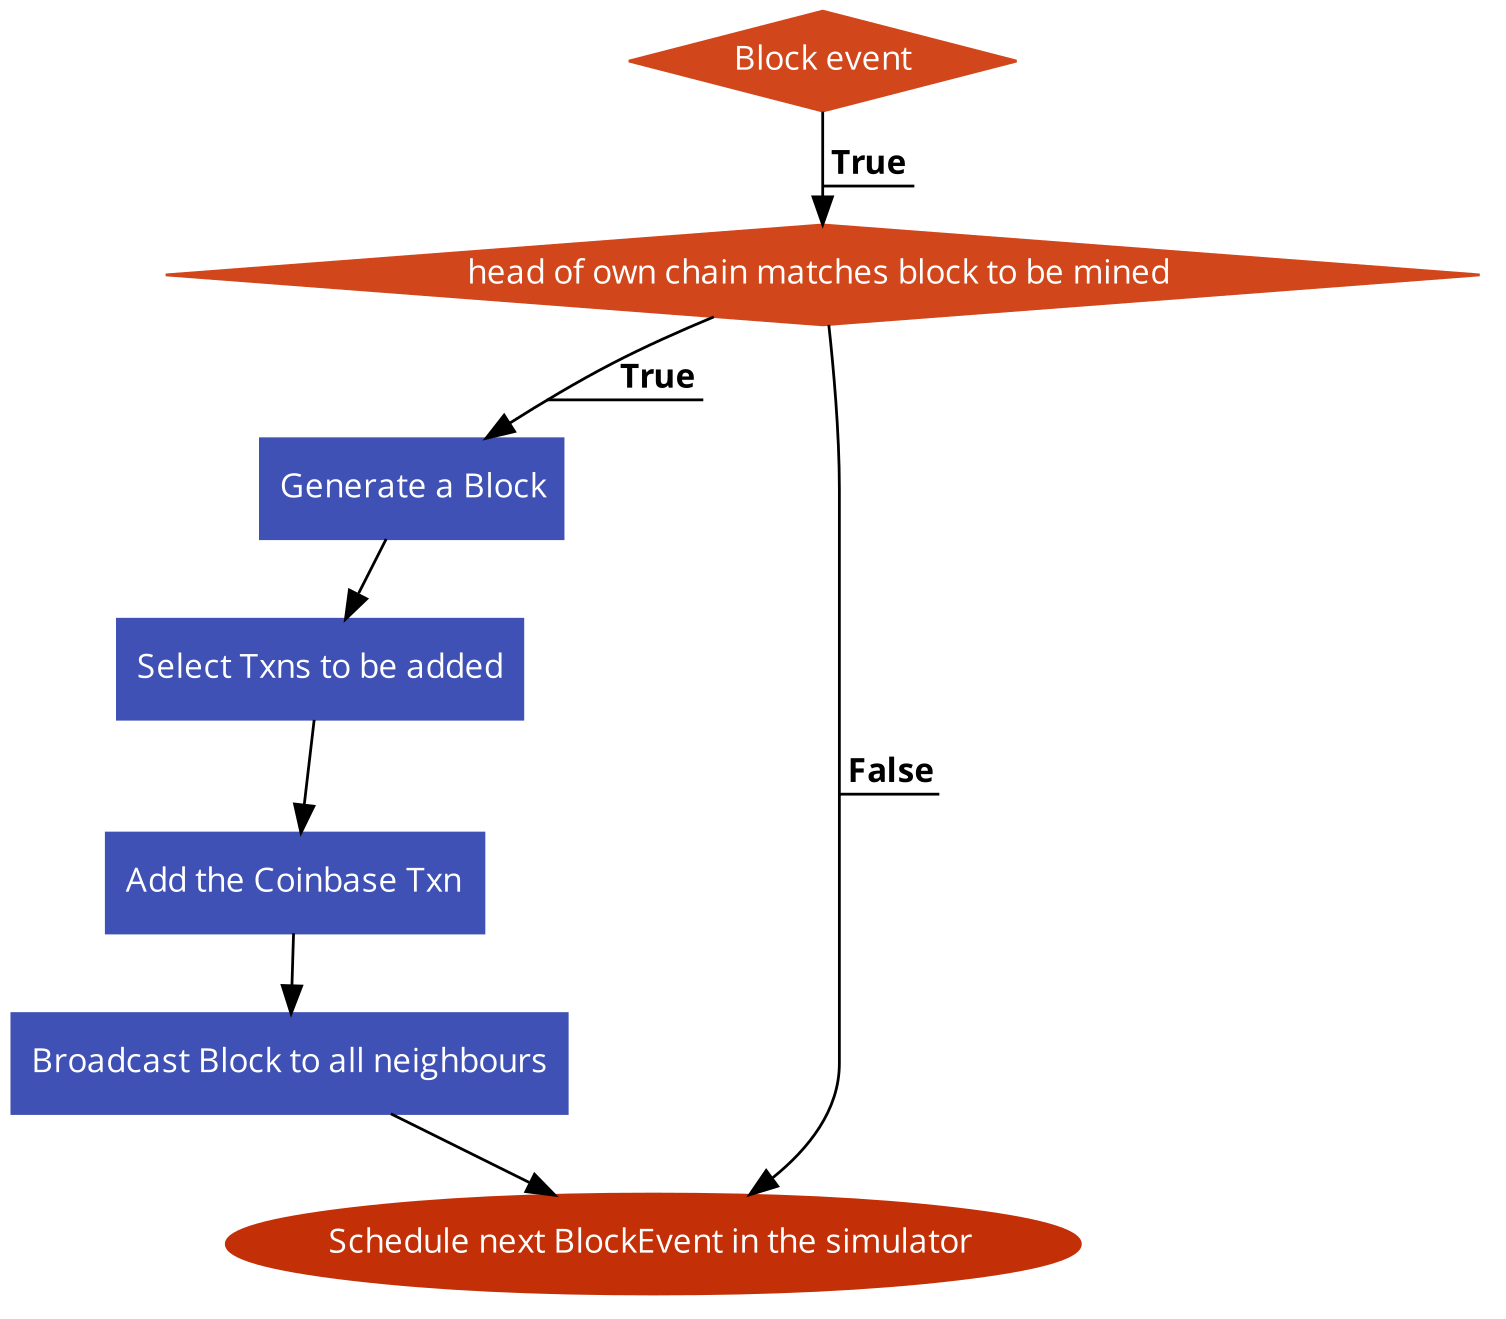
\includegraphics[width=6cm]{Block.png}

\rule[10px]{12cm}{1px}

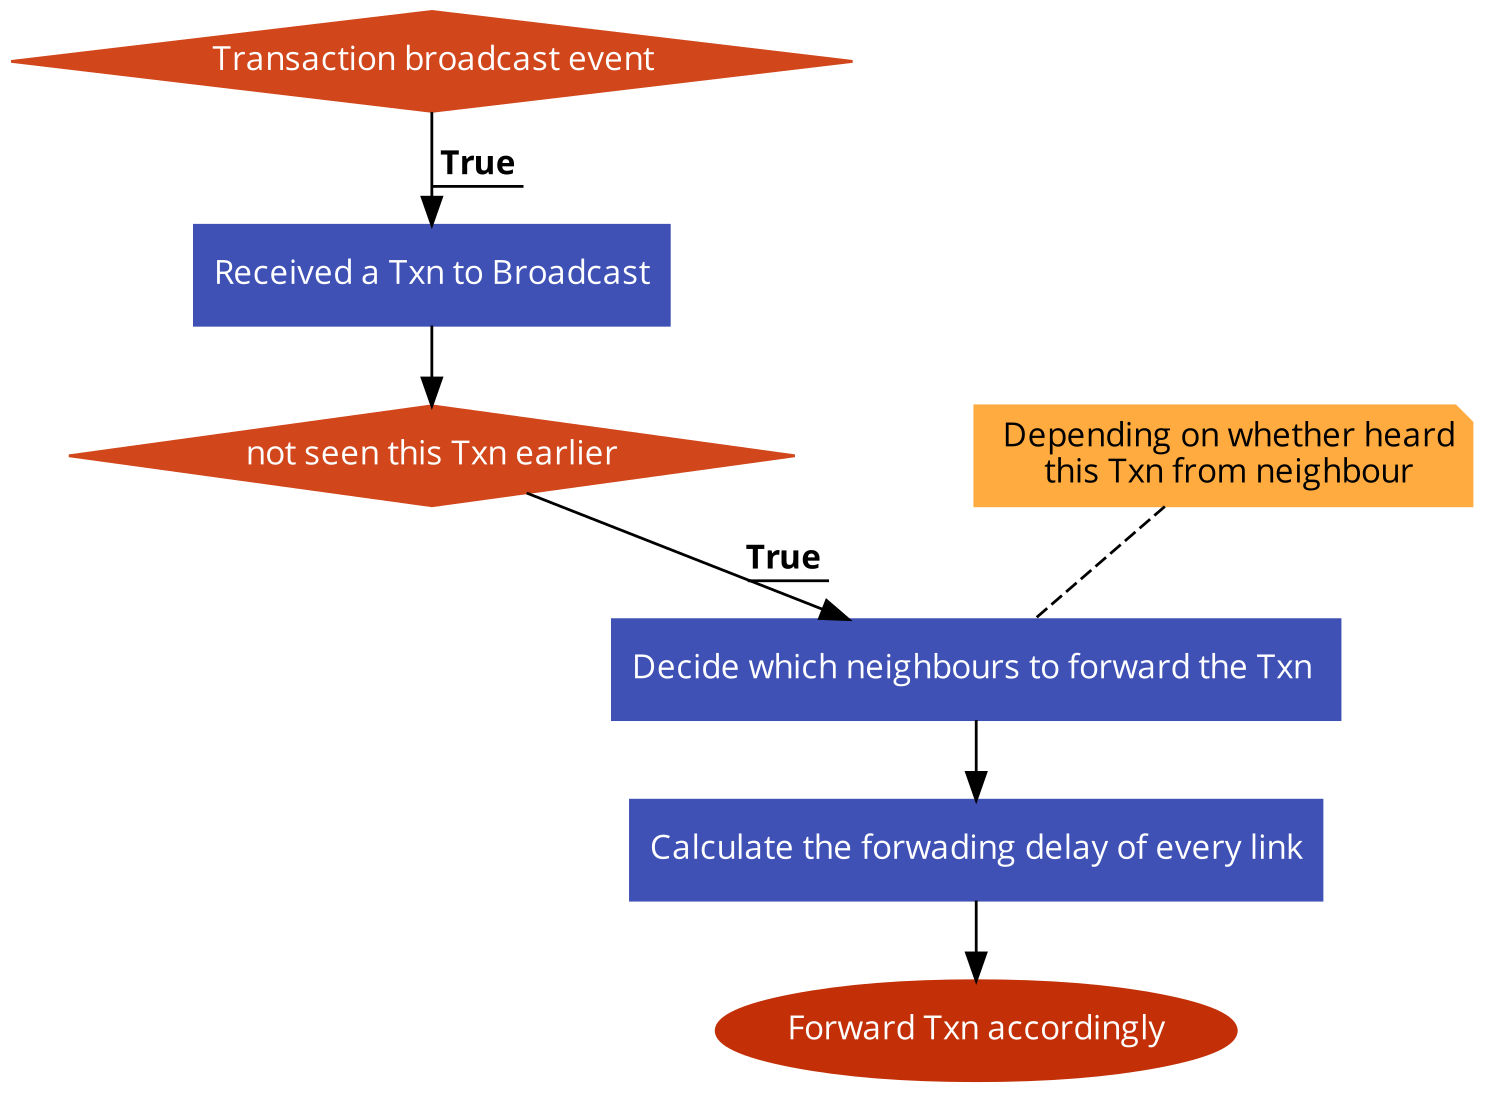
\includegraphics[width=6cm]{TxnBroadcast.png}
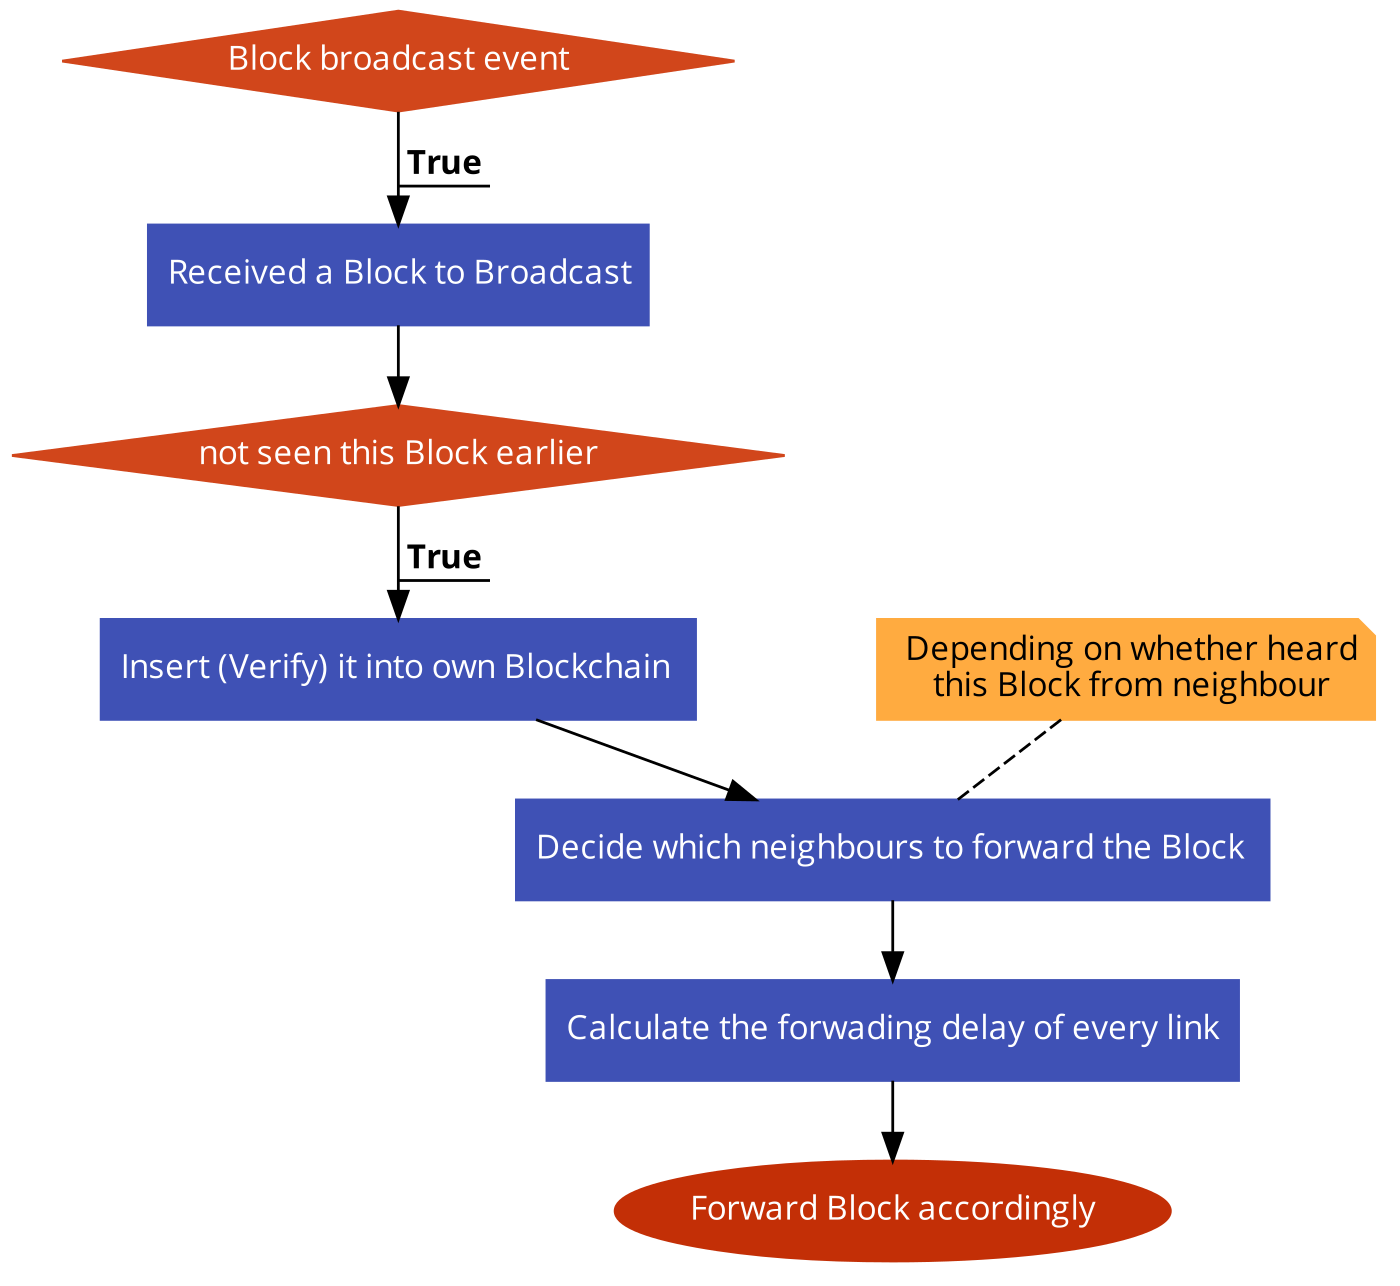
\includegraphics[width=6cm]{BlockBroadcast.png}

\section{Questions}

\subsection{ What are the theoretical reasons of choosing the exponential distribution?}

The process of finding a block is a poisson process, due to the semantics of the Proof of Work and Hashing threshold requirements.

Because the exponential distribution represents the difference between the two events in the poisson process, it is appropriate to use the exponential distribution to simulate the inter-arrival time gap between the blocks

\subsection{ Why is the mean of $d_{ij}$ inversely related to $c_{ij}$ ? Give justification for this choice.}

The amount of time a packet has to spend at a node $i$ is proportional to the number of packets ahead of it, and inversely proportional to the rate at which node $i$ is dispatching them to node $j$.
Since the latter is inversely related to link speed $c_{ij}$, hence $d_{ij} \propto \frac{1}{c_{ij}}$.



\end{document}